\section{Лекція 9: Основи використання функцій в Python}
 
 \subsection{Що таке функція?} 
\begin{frame}
% \frametitle{Логічні висновки}
Функція — частина програми, яка реалізує певний алгоритм і дозволяє звернення до неї з різних частин загальної (головної) програми.
\begin{figure}
  \begin{center}
    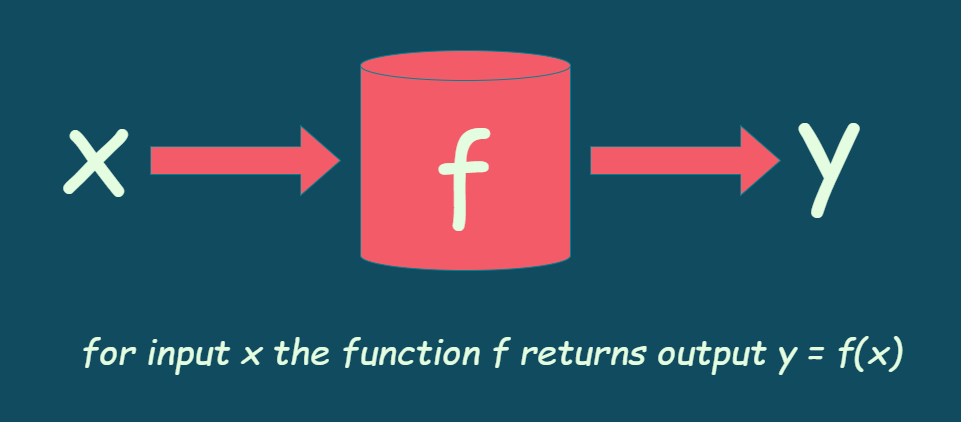
\includegraphics[width=\textwidth,height=0.4\textheight]{pictures/function.png}
  \caption{Функція}
\label{function}
  \end{center}
\end{figure}
\end{frame}

\begin{frame}
% \frametitle{Логічні висновки}
Приклад функції — \texttt{print}. При цьому \texttt{print} - посилання на об'єкт функцію (і воно може бути змінено, наприклад: \texttt{f = print}), а конструкція \texttt{print()} дозволяє запустити функцію на виконання.

\begin{center}
\large{DRY - Don't Repeat Yourself}
\end{center}

\normalsize Частини програми, що повторюються, слід розмістити в об'єкт функцію, а потім їх викликати в потрібних місцях.
\end{frame}

\begin{frame}
% \frametitle{Логічні висновки}
Синтаксис створення власної функції в Python:

\LARGE{def назва(список аргументів):

~~~~оператор 1

~~~~оператор 2

~~~~... 

~~~~оператор N }

\vspace{0.5cm}
\normalsize Аргумент всередині функції називається \textit{параметр}, а значення, що передається функції, підчас її виклику - \textit{аргумент}.
\end{frame}

 \subsection{Оператор return} 
\begin{frame}
% \frametitle{Логічні висновки}
Для того щоб вказати значення, яке повертає функція використовується оператор \texttt{return}.

\LARGE{def назва(список аргументів):

~~~~оператор 1

~~~~... 

~~~~оператор N

~~~~return значення }

\normalsize Щоб повернути декілька змінних використовується кортеж.

\end{frame}

\begin{frame}
% \frametitle{Логічні висновки}
\begin{itemize}
  \item В функціях можна викликати інші функції.
  \item Функції можна визначати всередині різних конструкції мови програмування (умовні оператори, цикли, інші функції тощо).
  \item Функції можна викликати всередині різних конструкції мови програмування (умовні оператори, цикли, інші функції тощо).
\end{itemize}

\end{frame}

\begin{frame}
% \frametitle{Логічні висновки}
Найбільший спільний дільник (НСД) чисел — найбільше натуральне число, на яке ці числа діляться без остачі. 

Алгоритм Євкліда для знаходження НСД чисел a та b:

\texttt{доки а != b} 

~~~~\texttt{знаходимо найбільше серед а та b}


~~~~\texttt{зменшуємо більше на величину меншого}

\texttt{виводимо а (або b)}

Швидкий алгоритм Євкліда:

\texttt{доки менше число більше 0}

~~~~\texttt{більше число = залишок від ділення на менше} 

\texttt{виводимо більше число}
\end{frame}

\begin{frame}
% \frametitle{Логічні висновки}
Якщо є функія \texttt{def func(a, b, c) ...} , то

\begin{itemize}
  \item При виклику функції позиції параметрів відповідають позиціям аргументів (позиційний запис аргументів) \texttt{func(1, 2, 3)}.
  \item При використанні іменованих аргументів можна передати параметрам функції значення із інших позицій аргументів \texttt{func(b=1, c=2, a=3)} або \texttt{func(1, c=2, =3)}.
\end{itemize}

\end{frame}

\subsection{Фактичні та формальні параметри} 
\begin{frame}
% \frametitle{Логічні висновки}
Якщо є функія \texttt{def func(a, b, c=1, d=2) ...} , то
\begin{itemize}
  \item \texttt{a} та \texttt{b} - фактичні параметри;
  \item \texttt{c} та \texttt{d} - формальні параметри;
  \item \texttt{1}  та \texttt{2} - значення за замовчуванням. 
\end{itemize}

Формальні параметри при виклику функції можна не вказувати, в цьому випадку використовуються значення за замовчуванням. Щоб задати значення формальних параметрів можна викликати функцію як \texttt{func(3, 4, c=2, d=1)} або як \texttt{func(3, 4, 2, 1)}.


\end{frame}

\subsection{Функції з довільним числом аргументів} 
\begin{frame}
% \frametitle{Логічні висновки}
\begin{itemize}
  \item \texttt{def func(*args) ...} - довільне число формальних аргументів (\texttt{args} - кортеж із довільного числа параметрів. 
  \item \texttt{def func(*args, par1=1, par2=2) ...}  - довільне число формальних аргументів та фактичні аргументи.
  \item \texttt{def func(*args, **kwargs) ...} - довільне число формальних аргументів та фактичних аргументів.
  \item \texttt{func(*args, p1=1, **kwargs) ...} - довільне число формальних і фактичних та фактичний аргумент.
   \item \texttt{def func(arg1, *args, p1=1, **kwargs) ...}  - довільне число формальних та фактичних, один формальний та конкретний фактичний аргумент.
\end{itemize}

\end{frame}

\subsection{Упаковка та розпаковка колекцій} 
\begin{frame}
% \frametitle{Логічні висновки}
\begin{itemize}
  \item Упаковка \texttt{x, *y = (1, 2, 3, 4)} або \texttt{*x, y = (1, 2, 3, 4)}
  \item Упаковка \texttt{x, *y = [1, "a", True, 4]} або \texttt{*x, y = "Hello!"}
  \item \texttt{*x = 1, 2, 3} - помилка
  \item Розпаковка списку \texttt{a = [1, 2, 3]} в кортеж \texttt{(*a,)}
  \item Розпаковка кортежу \texttt{a = -5, 5} в оператор \texttt{range(*a)}
  \item Щоб отримати список \texttt{*range(*a)}
  \item Розпаковка словника в словник \texttt{**d}
  \item Об'єднання словників \texttt{**d, **d1} 
\end{itemize}

\end{frame}
